\input{head.inc}

% Präambelbefehle für die Präsentation
\title[TET: Einführung]{Einführung}

\begin{document}
% 
% Frontmatter 
% 
%%%%%%%%%%%%%%%%%%%%%%%%%%%%%%%%%%%%%%%%%%%%%%%%%%%%%%%%%%%%%%%%%%%%%%%%%%%%%%%%%%%%%%%%%%%%%%%%%%%%%%%%%%%%%%%%%%%%%%%%%%%%% 

%% inserts the title page and the table of contents
\maketitle

% 
% Content 
% 
%%%%%%%%%%%%%%%%%%%%%%%%%%%%%%%%%%%%%%%%%%%%%%%%%%%%%%%%%%%%%%%%%%%%%%%%%%%%%%%%%%%%%%%%%%%%%%%%%%%%%%%%%%%%%%%%%%%%%%%%%%%%% 
\section{Einführung}

\begin{frame}
  \frametitle{Ausgangspunkt}

  \begin{block}{Die Maxwellschen Gleichungen}


    \begin{tabular}{l c c c l}
      differentielle Form & $\to$ & Satz & $\to$ & integrale Form \pause\\
      \hline
      $\divergenz \DFeld[v] = \laddichte{V}$ \pause& $\to$ & Gauss & $\to$ \pause& $\oiint\limits_{\oberfl(\volumen)}
                                                                            \DFeld[v] \cdot\intflaeche[v] =
                                                                            \iiint\limits_{\volumen} \laddichte{V}
                                                                            \intvolumen$\pause \\
      $\divergenz \BFeld[v] = 0$  \pause& $\to$ & Gauss & $\to$ \pause& $\oiint\limits_{\oberfl(\volumen)} \BFeld[v]\cdot
                                                               \intflaeche[v] = 0$\pause \\
      $\rotation \EFeld[v] + \dfrac{\partial
      \BFeld[v]}{\partial t} =\vec{0} $ \pause& $\to$ & Stokes & $\to$ \pause&
                                                                 $
                                                                             \oint\limits_{\oberfl(\Flaeche)}
                                                                             \EFeld[v]\cdot
                                                                             \intweg[v]
                                                                             =
                                                                             -
                                                                             \iint\limits_{\Flaeche}
                                                                             \dfrac{\partial
                                                                             \BFeld[v]}{\partial
                                                                             t}
                                                                             \cdot\intflaeche[v]
                                                                             =
                                                                             -
                                                                             \dfrac{\upd}{\upd
                                                                             t} \left[
                                                                             \iint\limits_{\Flaeche}
                                                                             \BFeld[v]
                                                                             \cdot\intflaeche[v]\right]
                                                                             $
                                                                             \pause \\
      $\rotation \HFeld[v] - \dfrac{\partial
      \DFeld[v]}{\partial t} = \StromDichte[v] $ \pause&
                                                                       $\to$ & Stokes & $\to$ \pause& $\oint\limits_{\oberfl(\Flaeche)} \HFeld[v]\cdot \intweg[v] = \iint\limits_{\Flaeche} \StromDichte[v] \cdot\upd \Flaeche[v] + \dfrac{\upd}{\upd t} \left[ \iint\limits_{\Flaeche} \DFeld[v] \cdot\intflaeche[v] \right]$\pause
    \end{tabular}

    
  \end{block}

  \begin{block}{Feldgrößen - Einheiten}
    \begin{itemize}[<+->]
    \item Elektrische Feldstärke $\EFeld[v]$  mit
      \(\left[\EFeld[v]\right] = \si{\volt\per\metre} \)
    \item Magnetische Feldstärke \(\HFeld[v] \) mit \(\left[\HFeld[v]\right] = \si{\ampere\per\metre} \)
    \item Elektrische Flussdichte \(\DFeld[v]\)  mit
      \(\left[\DFeld[v]\right] =
      \si{\coulomb\per\square\metre} =
      \si{\ampere\second\per\square\metre}\)
    \item Magnetische Flussdichte \(\BFeld[v]\) mit \(\left[\BFeld[v]\right] = \si{\tesla} = \si{\volt\second\per\square\metre} \)
    \end{itemize}
  \end{block}
\end{frame}

\begin{frame}
  \frametitle{Alternative Bezeichnungen}
  \begin{itemize}[<+->]
    \item Elektrisches Feld $\EFeld[v]$: - 
    \item Magnetisches Feld $\HFeld[v]$: in der Physik heute
      teilweise auch \alert{magnetische Anregung/Erregung} $\to$ Axiomatische
      Einführung
    \item Elektrische Flussdichte $\DFeld[v]$:
      \begin{itemize}[<+->]
        \item in der Physik heute
      teilweise auch \alert{elektrische Anregung/Erregung} $\to$ Axiomatische
      Einführung
      \item alternativ: \alert{dielektrische Verschiebung,
          Verschiebungsdichte, Verschiebungsflussdichte, D-Feld}
        \end{itemize}
      \item Magnetische Flussdichte $\BFeld[v]$:
        \begin{itemize}[<+->]
          \item in der Physik heute
      teilweise auch \alert{Magnetisches Feld} $\to$ Axiomatische Einführung
      \item alternativ:
        \alert{magnetische Induktion, Induktion, Flussdichte, B-Feld}
        \end{itemize}
  \end{itemize}    
      
  \end{frame}

  \begin{frame}
    \frametitle{Andere Größen - Einheiten}
    \begin{itemize}[<+->]
      \item Volumenladungsdichte $\laddichte{V}$:
        $\left[\laddichte{V}\right] = \si{\coulomb\per\cubic\metre} $
        (später auch Flächenladungsdichte und Linienladungsdichte)
        \item Stromdichte	\(\StromDichte[v]\) mit
          \(\left[\StromDichte[v]\right] =
          \si{\ampere\per\square\metre} \)
          \begin{itemize}[<+->]
		\item Allgemein Summe von drei Beiträgen:
		\begin{equation*}
			\StromDichte[v] = \StromDichte[v]_\mathrm{E} + \StromDichte[v]_\mathrm{L} + \StromDichte[v]_\mathrm{K}
		\end{equation*}
                \item Die eingeprägte Stromdichte
                  \(\StromDichte[v]_\mathrm{E}\) ist unabhängig vom
                  betrachtetem E-Feld.
                \item Die Leitungsstromdichte \(\StromDichte[v]_\mathrm{L}\) mit
		\begin{equation*}
			\StromDichte[v]_\mathrm{L} = \kappa \cdot \EFeld[v]
		\end{equation*}
		wird in aller Regel hier betrachtet. $\kappa$ ist die
                elektrische Leitfähigkeit; $\left[\kappa\right] =\si{\ampere\metre\per\volt\per\square\metre}=\si{(\ohm\metre)^{-1}}=\si{S\per\metre}$
                \item Die Konvektionsstromdichte \(\StromDichte[v]_K\) mit
		\begin{equation*}
			\StromDichte[v]_\mathrm{K} = \laddichte{V} \cdot \vec{v} \pointspacek
		\end{equation*}
		welches z.B. in Plasma vorkommt, spielt hier meist
                keine Rolle. 
\end{itemize}
              \end{itemize}
    \end{frame}
    \begin{frame}
      \frametitle{Materialgleichungen}
      \begin{itemize}[<+->]
        \item Die elektrischen Feldgrößen $\EFeld[v]$ und $\DFeld[v]$
          sind voneinander abhängig:
          
          $$
         \DFeld[v] = \varepsilon_0 \EFeld[v] +\vec{P}
                $$
           mit \alert{Polarisation} $\vec{P}$; $\left[\vec{P}\right] = \left[\DFeld[v]\right] =
           \si{\coulomb\per\square\metre}$
           \item Die magnetischen Feldgrößen $\HFeld[v]$ und
             $\BFeld[v]$ sind voneinander abhängig:

             $$
             \BFeld[v] = \mu_0  \left( \HFeld[v] + \Magnetisierung[v] \right)
             $$
             mit \alert{Magnetisierung} $\vec{M}$, $\left[\vec{M}\right] =
             \left[\vec{H}\right] = \si{\ampere\per\metre}$
             \item Ohne Materie (im \alert{Vakuum}) gibt es keine
               Polarisation und keine Magnetisierung. Es gilt
               $\DFeld[v] = \varepsilon_0 \EFeld[v]$ und
               $\BFeld[v] = \mu_0  \HFeld[v]$.
               \item Die \alert{Dielektrizitätskonstante/Permittivität des Vakuums}
                 $\varepsilon_0$ und die \alert{Permeabilität des
                   Vakuums} $\mu_0$ sind universelle Konstanten und
                 mit der \alert{Lichtgeschwindigkeit im Vakuum} $c$
                 verknüpft:
                 \begin{align*}
                   c & = \SI{299792458}{\metre\per\second} \approx
                       \SI{3e8}{\metre\per\second} \alert{\text{
                       also: } \SI{30}{cm / ns}}\\
                   \mu_0 & = 4\pi\cdot
                   10^{-7}\,\si{\volt\second\per(\ampere\metre)}\\
                   \varepsilon_0 & = \dfrac{1}{\mu_0  c^2} \approx
                   \SI{8,85e-12}{\ampere\second\per(\volt\metre)}
                   \text{ mit } \alert{c^2\varepsilon_0\mu_0 = 1} 
                   \end{align*}
               \end{itemize}
       \end{frame}

       \begin{frame}
         \frametitle{Materialgleichungen - homogene, lineare, isotrope
           Medien}
         \begin{itemize}[<+->]
           \item In aller Regel werden wir uns auf \alert{homogene,
               lineare, und isotrope Medien} beschränken
             \item Ein Medium ist \alert{homogen} bezüglich einer
               bestimmten Eigenschaft, wenn diese Eigenschaft nicht
               vom \alert{Ort} abhängt. 
               \item Ein Medium ist \alert{linear} bezüglich einer
                 bestimmten Eigenschaft und einer bestimmten Anregung,
                 wenn die Eigenschaft nicht von der \alert{Amplitude} der
                 Anregung abhängt (z.B. Federkonstante im Hookschen
                 Bereich)
                 \item Ein Medium ist \alert{isotrop} bezüglich einer
                   bestimmten Eigenschaft und einer bestimmten
                   Anregung, wenn die Eigenschaft unabhängig von der
                   \alert{Richtung} der Anregung ist (z.B. ist die
                   Polarisation in Kristallen häufig nicht isotrop
                   bezüglich einer elektrischen Anregung).
                   \item Es gelten dann die
                     \alert{Materialgleichungen für homogene,
                       lineare, und isotrope Medien}:
                     $$ \DFeld[v] =
                     \underbrace{\varepsilon_0\varepsilon_r}_{=\varepsilon}
                     \EFeld[v] \text{ und } \BFeld[v] =
                     \underbrace{\mu_0  \mu_r}_{=\mu} \HFeld[v] $$
                   \item Für Polarisation und Magnetisierung
              $$\vec{P} = \varepsilon_0(\varepsilon_r - 1) \vec{E}
              \text{ und }  \vec{M} = (\mu_r-1) \vec{H}$$
           \end{itemize}
         \end{frame}

         \begin{frame}
           \frametitle{Beiträge zur komplexen Permittivität}
           \begin{columns}[t]
             \begin{column}{.6\textwidth}
               
               \centering
               \onslide<+->{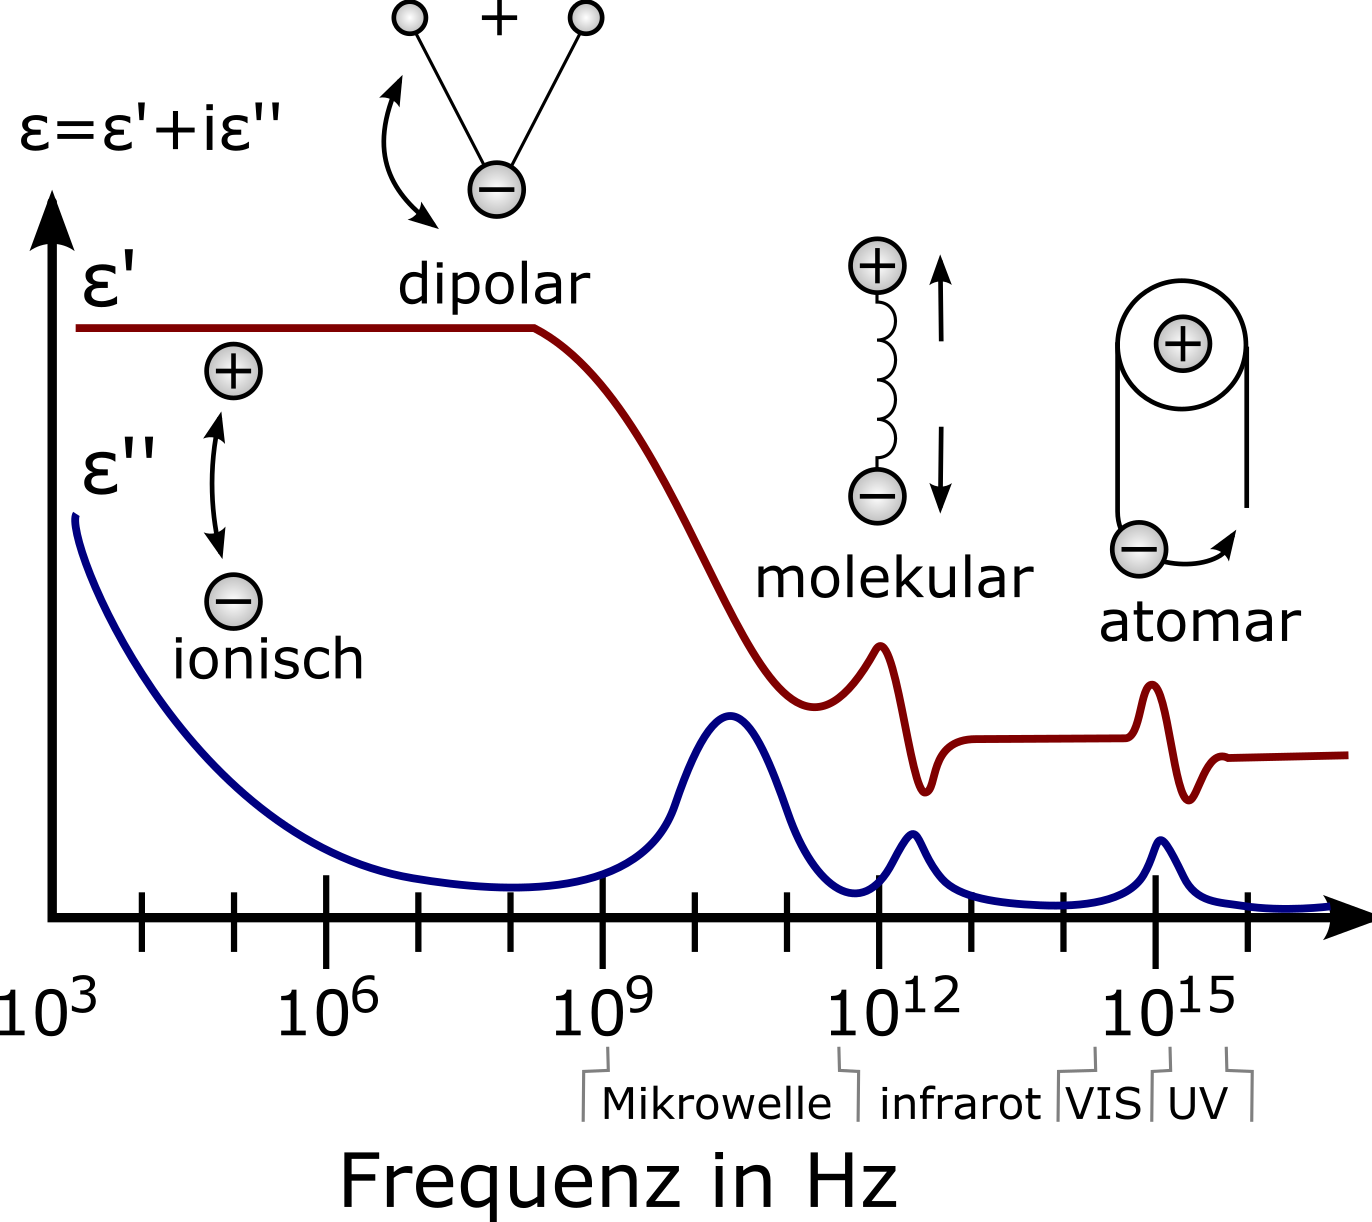
\includegraphics[width=\columnwidth]{Dielectric_responses_DE.png}
               {\tiny Quelle:  Prof. Kenneth A. Mauritz, derivative work: Cepheiden, Attribution, via Wikimedia Commons}}
             \end{column}
             \begin{column}{.4\textwidth}
               \begin{itemize}[<+->]
                 \item Grundsätzlich verschiedenes Verhalten bei
                   vorhandenen oder nicht vorhandenen Rückstellkräften
                   \item dipolar: Polare Moleküle (z.B. Wasser)
                     orientieren sich im Feld, keine Rückstellkraft
                     (nur thermische Bewegung) $\to$ Debye-Relaxation
                     \item molekular, atomar: Rückstellkräfte
                       vorhanden $\to$ harmonischer Oszillator
                       \item Dielektrische Spektroskopie $\to$
                         Aufklärung der Mechanismen
                 \end{itemize}
             \end{column}
           \end{columns}
         \end{frame}

\input{finalframe.inc}
\end{document}